\chapter{Faithful Witnesses in the Midst of Suffering (10:1--11:19)}

In the previous chapter, we read about the first six trumpets. Surely, the seventh trumpet\index{trumpets, seven!7@seventh trumpet} must be next. Yet before it sounds, Revelation pauses to present two visions: John is commissioned to prophesy again, and two witnesses\index{two witnesses} testify before the world. Only then does the seventh trumpet sound.

Why are these two visions placed here? Both reveal an essential truth: even as God's judgments\index{judgment} unfold, His people still bear the responsibility of witnessing to Him. Though suffering and persecution\index{persecution} may come, they are called to remain faithful to His Word and to testify to His truth until the kingdom of Christ is fully revealed.

From the heights, the eagle sees not only the judgments falling upon the earth, but also the witnesses who continue to proclaim God's truth amid the gathering darkness. Judgment does not silence their calling. Rather, their faithfulness shines all the more clearly against the shadows of a world opposed to God.

\section{John Is Commissioned to Prophesy Again}
\begin{ScriptureBox}

\item[10:1] Then I saw another mighty angel coming down from heaven. He was robed in a cloud, with a rainbow above his head; his face was like the sun, and his legs were like fiery pillars.

\item[10:2] He was holding a little scroll, which lay open in his hand. He planted his right foot on the sea and his left foot on the land,

\item[10:3] and he gave a loud shout like the roar of a lion. When he shouted, the voices of the seven thunders spoke.

\item[10:4] And when the seven thunders spoke, I was about to write; but I heard a voice from heaven say, ``Seal up what the seven thunders have said and do not write it down.''

\item[10:5] Then the angel I had seen standing on the sea and on the land raised his right hand to heaven.

\item[10:6] And he swore by him who lives for ever and ever, who created the heavens and all that is in them, the earth and all that is in it, and the sea and all that is in it, and said, ``There will be no more delay!

\item[10:7] But in the days when the seventh angel is about to sound his trumpet, the mystery of God will be accomplished, just as he announced to his servants the prophets.''

\item[10:8] Then the voice that I had heard from heaven spoke to me once more: ``Go, take the scroll that lies open in the hand of the angel who is standing on the sea and on the land.''

\item[10:9] So I went to the angel and asked him to give me the little scroll. He said to me, ``Take it and eat it. It will turn your stomach sour, but `in your mouth it will be as sweet as honey.'\,''
% NIV footnote for 10:9 (omitted; add as \footnote if wanted):
%   ``as sweet as honey'' --- Ezek. 3:3
% CHECK NIV: footnote reference quoted from memory; verify against Bible Gateway.

\item[10:10] I took the little scroll from the angel's hand and ate it. It tasted as sweet as honey in my mouth, but when I had eaten it, my stomach turned sour.

\item[10:11] Then I was told, ``You must prophesy again about many peoples, nations, languages and kings.''

\end{ScriptureBox}


\begin{figure}[htbp]
    \centering
    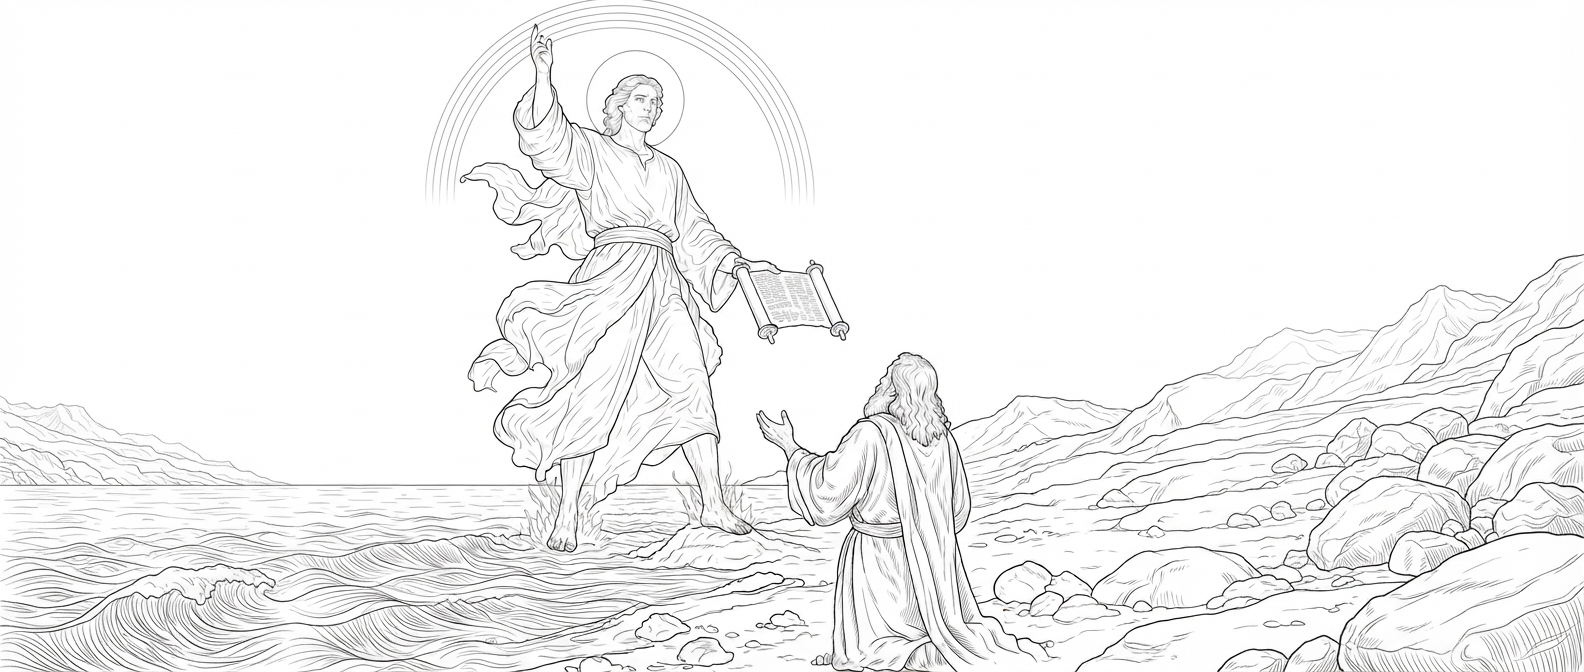
\includegraphics[
    width=1\textwidth,
    trim=200 0 200 0,
    clip]{images/small_scroll2.jpg}
\end{figure}

God's Word is sweet as honey in the mouth because it reveals His truth and brings comfort to those who receive it. Yet the same Word turns bitter in John's stomach, for proclaiming God's truth faithfully also means confronting judgment, suffering, and persecution\index{persecution}.

The sweetness and bitterness belong together. God's revelation is a gift, illuminating the darkness and offering hope to His people. But the messenger who receives that gift must also bear the burden of proclaiming it. The truth that comforts the faithful may expose the world's rebellion and provoke the hostility of those who refuse to hear it.

\begin{ReaderQuestion}
Why is God's Word both “sweet as honey” and bitter in the stomach? What does this image teach us about the joy and the cost of receiving and proclaiming God's truth?
\end{ReaderQuestion}

When John prepares to write down what the seven thunders have spoken, a voice from heaven commands him to seal up their words and not write them down. Not everything John hears or sees is to be disclosed. God determines what is revealed and what remains hidden.

Deuteronomy 29:29 expresses this principle: “The secret things belong to the LORD our God, but the things revealed belong to us and to our children forever” (NIV).

The heart of our faith does not lie in discovering every detail of the end times\index{end times}. It lies in trusting the God who governs history and faithfully receiving the truth He has chosen to reveal. There is a spiritual discipline in acknowledging the limits of our understanding. We are called to approach what remains hidden with humility and to devote ourselves to obeying what God has already made known.

John is then commanded to take the little scroll\index{scroll!little scroll} and eat it. Its sweetness and bitterness prepare him for the work that follows: he must prophesy again concerning many peoples, nations, languages, and kings. Receiving God's Word is not the end of his calling. He must carry that Word into the world, whatever the cost.

So it is with God's people in every generation. We do not receive His Word merely to satisfy our curiosity or comfort ourselves in private. We receive it so that we may live by it, proclaim it, and remain faithful to it—even when obedience brings sorrow.

\section{The Two Witnesses}\index{two witnesses}
\begin{ScriptureBox}

\item[11:1] I was given a reed like a measuring rod and was told, ``Go and measure the temple of God and the altar, with its worshipers.

\item[11:2] But exclude the outer court; do not measure it, because it has been given to the Gentiles. They will trample on the holy city for 42 months.

\item[11:3] And I will appoint my two witnesses, and they will prophesy for 1,260 days, clothed in sackcloth.''

\item[11:4] They are ``the two olive trees'' and the two lampstands, and ``they stand before the Lord of the earth.''
% NIV footnote for 11:4 (omitted; add as \footnote if wanted):
%   ``before the Lord of the earth'' --- Zech. 4:3,11,14
% CHECK NIV: footnote reference quoted from memory; verify against Bible Gateway.

\item[11:5] If anyone tries to harm them, fire comes from their mouths and devours their enemies. This is how anyone who wants to harm them must die.

\item[11:6] They have power to shut up the heavens so that it will not rain during the time they are prophesying; and they have power to turn the waters into blood and to strike the earth with every kind of plague as often as they want.

\item[11:7] Now when they have finished their testimony, the beast that comes up from the Abyss will attack them, and overpower and kill them.

\item[11:8] Their bodies will lie in the public square of the great city---which is figuratively called Sodom and Egypt---where also their Lord was crucified.

\item[11:9] For three and a half days some from every people, tribe, language and nation will gaze on their bodies and refuse them burial.

\item[11:10] The inhabitants of the earth will gloat over them and will celebrate by sending each other gifts, because these two prophets had tormented those who live on the earth.

\item[11:11] But after the three and a half days the breath of life from God entered them, and they stood on their feet, and terror struck those who saw them.
% NIV footnote for 11:11 (omitted; add as \footnote if wanted):
%   ``breath'' --- Or Spirit (see Ezek. 37:5,14)
% CHECK NIV: footnote wording quoted from memory; verify against Bible Gateway.

\item[11:12] Then they heard a loud voice from heaven saying to them, ``Come up here.'' And they went up to heaven in a cloud, while their enemies looked on.

\item[11:13] At that very hour there was a severe earthquake and a tenth of the city collapsed. Seven thousand people were killed in the earthquake, and the survivors were terrified and gave glory to the God of heaven.

\end{ScriptureBox}

\subsection{The Temple Is Measured, and the Holy City Is Trampled}\index{holy city}\index{temple}

Biblical visions sometimes depict the measuring of a temple\index{temple} or a city. Ezekiel\index{Ezekiel} 40--48 describes the measuring of the temple, while Zechariah\index{Zechariah} 2:1--5 records a vision in which Jerusalem\index{Jerusalem} is measured. Such imagery can signify God's recognition of what belongs to Him, its distinction as holy, and His protective claim over it.

In Revelation 11, John is told to measure God's temple, the altar\index{altar}, and those who worship\index{worship} there. The outer court, however, is excluded from the measurement and handed over to the Gentiles, who will trample the holy city\index{holy city} for forty-two months.

The image holds two truths together. God's people belong to Him, yet they may still suffer persecution\index{persecution} on earth. Being known by God does not mean being spared every trial. His people may be oppressed, their worship challenged, and their witness resisted, even as they remain His own.

How long will this oppression last? Several visions in Scripture use periods of time that correspond to one another: “forty-two months” (Revelation 11:2), “1,260 days\index{1,260 days}” (Revelation 11:3), and “a time, times and half a time\index{time, times, and half a time}” (Revelation 12:14). If a year is reckoned as twelve months of thirty days each, these expressions correspond to three and a half years.

Christian interpreters differ over how these periods should be understood and applied. Some read them as specific future periods, while others interpret them symbolically or in relation to the wider history of God's people. I discuss these views in the appendix, “How Long Will the Great Tribulation\index{Great Tribulation} Last? The Seventy Sevens\index{seventy sevens (Daniel 9)} of Daniel\index{Daniel}.”

Whatever interpretive approach one adopts, the period is significant in one essential respect: the time of suffering is limited. The forces that oppose God do not possess unlimited authority. The holy city\index{holy city} may be trampled, and the witnesses may be attacked, but their enemies cannot determine the final course of history. Their time is bounded by the sovereignty of God.

\begin{figure}[htbp]
    \centering
    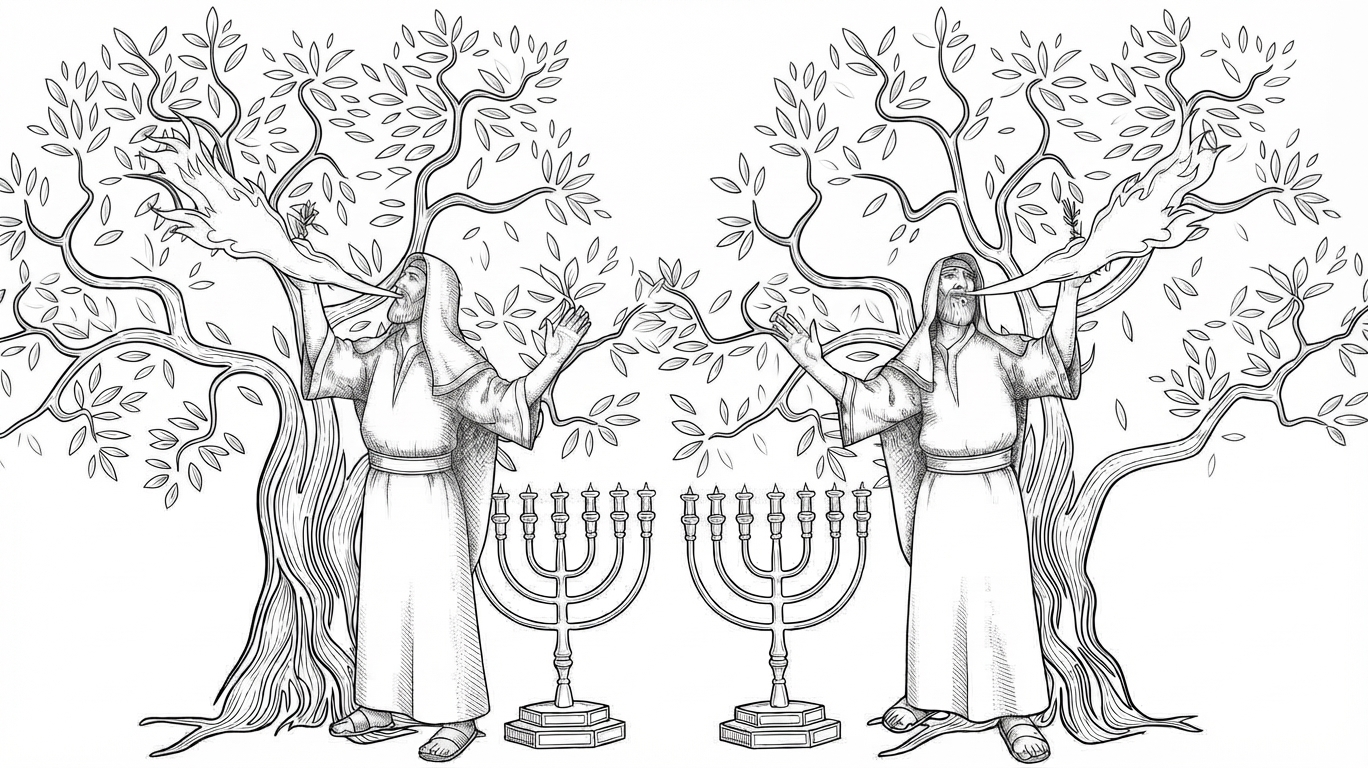
\includegraphics[
    width=1\textwidth,
    trim=0 0 0 0,
    clip]{images/two_witnesses.jpg}
\end{figure}

\subsection{Who Are the Two Witnesses?}\index{two witnesses}

John's vision draws extensively upon the Old Testament. Recognizing these connections helps us understand both the imagery and the theological meaning of the two witnesses\index{two witnesses}, as shown in Table \ref{tab:rev11-ot-background}.

{
\small
\renewcommand{\arraystretch}{1}

\begin{longtable}{
    @{}
    >{\raggedright\arraybackslash}p{0.24\textwidth} |
    >{\raggedright\arraybackslash}p{0.26\textwidth} |
    >{\raggedright\arraybackslash}p{0.40\textwidth}
    @{}
}
\caption{Old Testament background to Revelation 11}
\label{tab:rev11-ot-background} \\
\hline
\textbf{Revelation 11} & \textbf{Old Testament} & \textbf{Significance} \\
\hline
\endfirsthead

\multicolumn{3}{@{}l}{\small\itshape Table~\thetable\ (continued)} \\
\hline
\textbf{Revelation 11} & \textbf{Old Testament} & \textbf{Significance} \\
\hline
\endhead

\hline
\endfoot

\hline
\endlastfoot

The two witnesses
& Deuteronomy 19:15
& The principle that a matter is established by two or three witnesses \\
\hline
The two olive trees
& Zechariah 4:1--14
& The olive trees and lampstand in Zechariah's vision \\
\hline
The two lampstands
& Zechariah 4; Revelation 1:20
& Witness and the people of God \\
\hline
Fire from their mouths
& Jeremiah 5:14
& The power of God's word to pronounce judgment \\
\hline
The heavens shut
& 1 Kings 17:1
& Elijah's proclamation of drought \\
\hline
Water turned to blood
& Exodus 7:14--25
& Moses and the first plague upon Egypt \\
\hline
Various plagues
& Exodus
& The plagues through which God judged Egypt \\
\hline
The beast from the Abyss
& Daniel 7
& Political power in opposition to God \\
\hline
Sodom and Egypt
& Genesis; Exodus
& A corrupt and oppressive world that resists God and persecutes His people \\
\hline
Resurrection
& Ezekiel 37
& God's power to restore life to the dead \\
\hline
Taken up to heaven in a cloud
& Daniel 7:13; 2 Kings 2
& Divine glory and being taken up into heaven \\

\end{longtable}
}

\normalsize

These Old Testament connections provide a foundation for considering the different interpretations proposed by biblical scholars. The identity of the two witnesses\index{two witnesses} has been understood in several ways, as shown in Table \ref{tab:two-witnesses}.

{
\small
\renewcommand{\arraystretch}{1}

\begin{longtable}{
    @{}
    >{\raggedright\arraybackslash}p{0.35\textwidth} |
    >{\raggedright\arraybackslash}p{0.61\textwidth}
    @{}
}
\caption{Who are the two witnesses?}
\label{tab:two-witnesses} \\
\hline
\textbf{Proposed Identity} & \textbf{Principal Reasons} \\
\hline
\endfirsthead

\multicolumn{2}{@{}l}{\small\itshape Table~\thetable\ (continued)} \\
\hline
\textbf{Proposed Identity} & \textbf{Principal Reasons} \\
\hline
\endhead

\hline
\endfoot

\hline
\endlastfoot

Enoch and Elijah
& Both are described in Scripture as having been taken by God without an account of their ordinary deaths. \\
\hline
Moses and Elijah
& The signs involving fire, drought, and plagues recall the ministries of Elijah and Moses. Both also appear together at the Transfiguration of Jesus.\footnote{See the commentaries by Grant R. Osborne and John MacArthur.} \\
\hline
Two actual individuals raised up by God in the end times
& The detailed sequence of their preaching, death, resurrection, and ascent to heaven is understood as describing two specific future witnesses.\footnote{This view is held by a number of premillennial interpreters, including John MacArthur.} \\
\hline
The faithful church and people of God
& The imagery of the olive trees and lampstands is interpreted symbolically, representing the church's witness to the world.\footnote{See G. K. Beale and Craig R. Koester.} \\

\end{longtable}
}


\normalsize

These interpretations differ, but they all seek to account for the Old Testament imagery and the role of the witnesses in God's unfolding plan. The text does not explicitly name the two witnesses\index{two witnesses}, so it is wise to distinguish what the vision states directly from the conclusions interpreters draw from it.

Whatever their precise identity, their calling is unmistakable: they bear witness to God in a world that resists His truth. Their prophetic ministry recalls Moses\index{Moses} and Elijah\index{Elijah}, while the lampstand\index{lampstands} imagery connects their witness with the people of God. They proclaim the truth, confront evil, and remain faithful until their appointed testimony is complete.

Their story also overturns the world's measure of victory. The beast\index{beast} appears to prevail when it kills them, and the inhabitants of the earth celebrate their deaths. Yet the beast's triumph is temporary. God restores the witnesses to life and calls them into heaven. What appears to be defeat in the eyes of the world cannot overturn God's purpose.

\begin{ReaderQuestion}
The two witnesses are killed by the beast, and the inhabitants of the earth rejoice over their deaths. Today, might we also be tempted to remain silent about our faith because we fear how others will react? What can help us remain faithful to Christ?
\end{ReaderQuestion}

\subsection{What Do the Second and Third Woes Include?}\index{woes, three}

\begin{ScriptureBox}

% Insert the licensed NIV text of Revelation 11:14.
\item[11:14] \textit{The second woe has passed; the third woe is coming soon.}

\end{ScriptureBox}

The second woe\index{woes, three} encompasses the judgment associated with the sixth trumpet\index{trumpets, seven!6@sixth trumpet}, together with the vision of the two witnesses\index{two witnesses}. The third woe begins with the sounding of the seventh trumpet\index{trumpets, seven!7@seventh trumpet}. See Figure~\ref{fig:trumpets_woes}.

This transition reminds us that the visions in Revelation are not simply a sequence of disasters. Between the trumpets, John is shown the calling and suffering of God's witnesses. The judgments reveal God's opposition to evil, while the witnesses reveal the faithfulness He calls forth from His people. Even as the world is shaken, the testimony of God continues.

\section{The Seventh Trumpet Sounds}\index{trumpets, seven!7@seventh trumpet}

\begin{ScriptureBox}

\item[11:15] The seventh angel sounded his trumpet, and there were loud voices in heaven, which said:\\
\hspace*{1em}``The kingdom of the world has become\\
\hspace*{2em}the kingdom of our Lord and of his Messiah,\\
\hspace*{2em}and he will reign for ever and ever.''

\item[11:16] And the twenty-four elders, who were seated on their thrones before God, fell on their faces and worshiped God,

\item[11:17] saying:\\
\hspace*{1em}``We give thanks to you, Lord God Almighty,\\
\hspace*{2em}the One who is and who was,\\
\hspace*{1em}because you have taken your great power\\
\hspace*{2em}and have begun to reign.

\item[11:18] \hspace*{1em}The nations were angry,\\
\hspace*{2em}and your wrath has come.\\
\hspace*{1em}The time has come for judging the dead,\\
\hspace*{2em}and for rewarding your servants the prophets\\
\hspace*{1em}and your people who revere your name,\\
\hspace*{2em}both great and small---\\
\hspace*{1em}and for destroying those who destroy the earth.''

\item[11:19] Then God's temple in heaven was opened, and within his temple was seen the ark of his covenant. And there came flashes of lightning, rumblings, peals of thunder, an earthquake and a severe hailstorm.

\end{ScriptureBox}

When the seventh trumpet\index{trumpets, seven!7@seventh trumpet} sounds, heaven's first announcement is not another description of disaster. It is a proclamation of the certainty of Christ's reign: the kingdom of the world has become the kingdom of our Lord and of His Messiah\index{Messiah}, and He will reign for ever and ever.

The twenty-four elders\index{twenty-four elders} fall facedown before God in worship. They give thanks to the Lord God Almighty, who has taken His great power and begun to reign. The nations have raged, but God's wrath\index{wrath of God} has come. The time has arrived to judge the dead, to reward His servants the prophets and His holy people—all who fear His name, both great and small—and to destroy those who destroy the earth.

The seventh trumpet\index{trumpets, seven!7@seventh trumpet} therefore turns our attention beyond the partial judgments that have marked the earlier trumpets. The repeated limitation to a third gives way to the announcement of God's final purpose: evil will be judged, His faithful servants will be rewarded, and His reign will be openly established.

The opening of God's heavenly temple\index{temple} and the appearance of the ark of His covenant deepen this vision. The ark recalls God's covenant faithfulness and His presence among His people. Even amid lightning, rumblings, thunder, an earthquake\index{earthquake}, and a great hailstorm, the covenant-keeping God remains at the center of the vision.

The seventh trumpet\index{trumpets, seven!7@seventh trumpet} announces the certainty of the kingdom, though Revelation will continue to unfold the events and visions surrounding the final conflict. In the next chapter, we will look more deeply into the spiritual nature of that conflict and see how the powers that oppose God move toward their ultimate defeat.

The message to the church is clear: remain faithful in the midst of suffering. The witnesses may be despised, attacked, and even killed, but their testimony is not in vain. The beast\index{beast} does not have the final word. Christ does. The kingdom of the world will not remain forever in the hands of those who resist God; it belongs to the Lord and His Messiah\index{Messiah}, whose reign endures for ever and ever.

\begin{ReaderQuestion}
If God is calling you to be a faithful witness in your family, church, workplace, or circle of friends, what might He be asking you to uphold, change, or speak about with courage?
\end{ReaderQuestion}
